

A total of 488 sources were initially identified, and after applying selection criteria and expanding through exploration of grey literature, we ended up with 156 relevant results. This section presents these results organized according to the predefined research questions, referencing the identified tools by their assigned IDs, as can be seen in the Tables \ref{tab:results} and \ref{tab:results_grey} The complete analysis can be found in a Technical Report: \footnote{Technical Report: https://tinyurl.com/mtzzy2um} , which contains all sources retrieved and how they answer each RQ. 

\begin{figure}[h!]
\begin{center}
    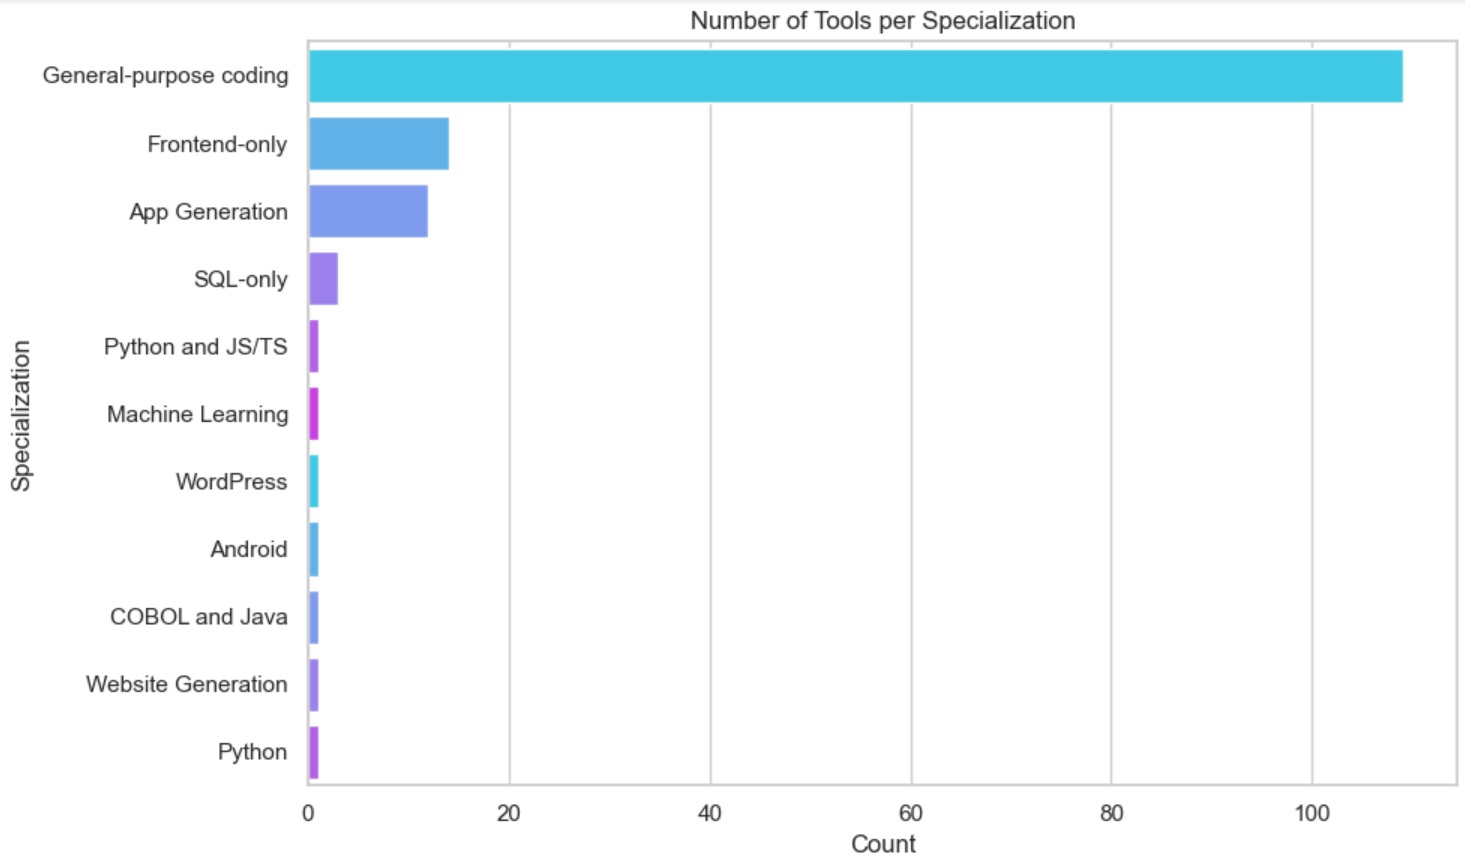
\includegraphics[width=0.48\textwidth]{figures/specialization-class.jpg}
    \caption{Distribution of tools across thematic clusters}
    \label{fig:tools_distribution}
\end{center}
\end{figure}

\subsection{RQ1a: Where can these solutions be found?}

The identified tools and technologies were primarily found across diverse channels and platforms, including official websites, dedicated repositories such as GitHub, academic databases, and specialized industry blogs. Prominent platforms for hosting these solutions include GitHub (e.g., Copilot [A01, A14, A19], StructCoder [A08]), official project websites (e.g., IBM Watsonx [A22, A35], Ansible Lightspeed [A05]), and specialized AI repositories like Hugging Face (e.g., CodeFuse-13B [A07], MarianCG [A17]). Grey literature tools such as CodeVista [A24] and Amazon Q [A25] are typically available through company websites or commercial cloud services. 

Additionally, a significant portion of grey literature is located on product and open-source portals associated with IDEs and CLIs. For instance, self-hosted assistants like Tabby [S029] on Github, editor-integrated agents such as Continue [S026] and Aider [S060], and vendor pages for JetBrains AI [S036], Gemini Code Assist [A21], and Amazon Q Developer CLI [S046]. 


\subsection{RQ1b: How can these solutions be used?}

These solutions can be categorized based on their usage contexts as follows:

\textbf{General-purpose tools:} These tools (e.g., Copilot [A01, A14, A33], Tabnine [A01], Gemini Code Assist [A21]) are integrated within Integrated Development Environments (IDEs) and are widely utilized for code generation, completion, debugging, and documentation generation across various programming languages. The general-purpose segment also includes IDE-native assistants and editor extensions such as Cursor [S001], Windsurf [S008], Zed AI [S097], Sourcegraph Cody [S014], Refact [S025], Continue [S026], and Aider [S060]. These tools offer edits, multi-file reasoning, and git-aware workflows.

\textbf{Frontend-only solutions:} Tools such as UI Pilot [S006], GitWit [S007], and Rapidpages [S084] specifically target frontend development tasks, aiding developers with tasks related to interface design and user experience improvements. This niche also encompasses design-to-code and UI generation platforms, such as v0 [S111], Uizard [S089], Kombai [S087], Magic Patterns [S085], and Galileo AI [S113], which translate wireframes or natural language prompts into React/HTML components and design artifacts.

\textbf{Application generation tools:} Replit [A28], OpenHands [S000], and GPT Web App Generator [S080] support developers in quickly creating functional prototypes or complete web and mobile applications directly from natural language descriptions. Other end-to-end generators include Bolt.new [S076], Lovable [S078], Second.dev [S104], Make Real [S081], SoftGen [S074], and Mage [S083], which scaffold multi-page apps, backends, or agents with runnable code and deployment recipes.

\textbf{Task automation solutions:} Ansible Lightspeed [A05], Grit [S065], and Shell Whiz [S054] facilitate automation of repetitive or configuration-related tasks, improving efficiency in software deployment and system management. At the CLI/infrastructure layer, Amazon Q Developer CLI [S046] and DevOpsGPT [S067] bring natural-language tasking to terminals and pipelines, while Warp [S057] and GitFluence [S055] accelerate command and Git workflow authoring.

These categories mirror the practical usage patterns reported in a recent qualitative study (\cite{klemmer2024using}), where developers highlighted use cases ranging from ideation to security mitigation practices.

\subsection{RQ1c: What is the access and usage model for these solutions and costs?}

The majority of identified tools operate under subscription or freemium models, offering limited free access to attract users. Copilot [A01, A14, A19, A23, A33] and Tabnine [A01, S030] typically follow subscription-based licensing. Platforms such as Amazon Q [A25, S041, S046] and IBM Watsonx [A22, A35] require authentication via respective cloud accounts with variable pricing based on usage. Open-source models like Code LLaMA and CodeFuse-13B [A07] are freely accessible under permissive licenses. Some simpler web-based tools like AI Code Converter [S092] offer free use, monetizing through advertisements.

Enterprise offerings increasingly provide on-premises or air-gapped deployments (e.g., Tabnine Enterprise and Ansible Lightspeed with on-prem options), while IDE add-ons like JetBrains AI Assistant follow per-seat subscriptions; Google’s Gemini Code Assist mixes a no-cost tier in Android Studio with paid tiers (Business/Enterprise) for advanced context windows and CLI features.


\subsection{RQ1d: What limitations must be considered for adopting these solutions?}

Several limitations should be considered:

\textbf{Technical limitations:} Many generative tools struggle with context awareness and producing accurate, secure code in complex scenarios (e.g., Copilot [A14, A19], CodeFuse-13B [A07]). Previous empirical studies (\cite{perry2023users, ji2024cybersecurity}) report elevated rates of vulnerabilities in AI-assisted or AI-generated code and reduced security quality among users relying on assistants.

\textbf{Operational constraints:} Most solutions, such as those from Google Cloud [A32], require stable internet connectivity and may present integration complexities within the existing infrastructure. Dependence on external APIs also imposes usage rate limits. Where data residency or connectivity constraints apply, organizations may favor self-hosted or hybrid alternatives (e.g., Tabby [S029]) and enterprise products with on-premises modes.

\textbf{Legal and ethical concerns:} Solutions handling sensitive data must comply with regulations such as GDPR. Tools that utilize external APIs or cloud-based services (IBM Watsonx [A35], Amazon Q [A25]) may pose challenges related to data privacy and intellectual property rights.

\subsection{RQ1e: What is the maturity level of these solutions?}

The identified solutions vary significantly in maturity:

\textbf{Production-ready:} Widely adopted commercial solutions such as Copilot [A01, A14, A19], Tabnine [A01], and Vertex AI [A32] demonstrate high maturity and are extensively validated in real-world settings. Other enterprise-grade assistants, such as JetBrains AI [S036], Amazon Q Developer/CLI [S041, S046], and Gemini Code Assist [A21], are also available and documented as stable, with integration across multiple IDEs.

\textbf{Experimental or beta phase:} Tools like ASPIRE [A10] and Spec2Code [A02] are in experimental stages with ongoing validation through academic and industrial case studies. Open research models for code (e.g., CodeFuse-13B [A07]) report internal deployments and evaluations.

\subsection{RQ1f: Is there technical documentation, support, or an active community?}

Most solutions provide comprehensive documentation, tutorials, and user manuals through their official channels. Copilot [A14, A19, A23, A33], IBM Watsonx [A35], and Google Cloud Vertex AI [A32] have extensive support channels, including forums, GitHub issue trackers, and customer support. 

Developer ecosystems around Continue [S026], Aider [S060], and Tabby [S029] are active and open-source-centric (docs, GitHub issues, Slack/Discord) while vendor ecosystems for JetBrains AI and Gemini Code Assist provide in-product guides, release notes, and enterprise onboarding materials.

\subsection{RQ1g: What types of target users typically engage with these solutions?}

These tools target various roles within software engineering:

\textbf{Developers and programmers:} Primary users for tools like Copilot [A01, A14], Tabnine [A01], and Gemini Code Assist [A21].

% \textbf{Testers and QA engineers:} Solutions such as ASPIRE [A10] and Calico [A06] specifically target roles involved in testing, debugging, and defect detection.

\textbf{DevOps professionals:} Task automation tools like Ansible Lightspeed [A05] and Grit [S065] benefit DevOps and infrastructure engineers directly. It must be stated that these tools do generate code and/or configuration files that automate the DevOps activities.

\subsection{RQ1h: Is there collaboration with industry through case studies or experiments?}

Some of the solutions have documented industry collaboration:

\textbf{Industrial case studies:} Tools like Spec2Code [A02] have empirical validation through industrial cases (e.g., Scania). CodeFuse-13B [A07] has been validated within AntGroup's software development processes.

\textbf{Large-scale user studies:} Ansible Lightspeed [A05] and Copilot [A14] have extensive user-based empirical studies highlighting practical industry validation and acceptance.




\begin{table*}[ht]
\centering
\caption{Technologies Employed in Software Construction: Initial Primary Sources}
\label{tab:results}
\begin{tabular}{|c|p{5cm}|p{2.5cm}||c|p{5cm}|p{2.5cm}|}
\hline
ID & Name / Technologies Identified & Specialization & ID & Name / Technologies Identified & Specialization \\
\hline
A01 & Github Copilot, Tabnine, Replit Ghostwriter, Codeium, JetBrainsAI Assistant, Kite, Visual Studio IntelliCode, Amazon CodeWhisperer, Sourcegraph Cody, Atlassian Intelligence, StarCoder, Chat-GPT & General-purpose & A21 & Gemini Code Assist & General-purpose \\
\hline
A02 & spec2code & General-purpose & A22 & IBM Watsonx & General-purpose \\
\hline
A03 & NL2Code & General-purpose & A23 & ChatGPT, Copilot & General-purpose \\
\hline
A04 & Proposed Methodology (Alpha Codium, LangChain, LangGraph, GPT), ChatGPT, Claude, ChatPDF, Perplexity & General-purpose & A24 & CodeVista & General-purpose \\
\hline
A05 & Ansible Lightspeed & Task Automation / Python & A25 & Amazon Q & General-purpose \\
\hline
A06 & Calico & General-purpose & A26 & ELEKS’ generative AI software development & General-purpose \\
\hline
A07 & CodeFuse-13B & General-purpose & A27 & ChatGPT, Copilot & General-purpose \\
\hline
A08 & StructCoder & General-purpose & A28 & Replit & App Generation \\
\hline
A09 & Codex, Copilot, PaLM2 (Pathways Language Model) & General-purpose & A29 & Shreds.AI & General-purpose \\
\hline
A10 & ASPIRE & General-purpose & A30 & ChatGPT, Copilot & General-purpose \\
\hline
A11 & Software Engineer GPT (Tailored GPT) & General-purpose & A31 & Jupyter AI & General-purpose \\
\hline
A12 & GPT-4 plus DSL & General-purpose & A32 & Google Cloud Vertex AI, Gemini models & ML \\
\hline
A13 & AskIt & General-purpose & A33 & Copilot & General-purpose \\
\hline
A14 & GitHub Copilot AI & General-purpose & A34 & Konveyor AI & General-purpose \\
\hline
A15 & The Programmer’s Assistant & General-purpose & A35 & IBM watsonx.ai & General-purpose \\
\hline
A16 & UniXcoder, CodeGPT, and InCoder & General-purpose & A36 & InCoder & General-purpose \\
\hline
A17 & MarianCG & General-purpose & A37 & Google Generative AI SDK for Kotlin & Android \\
\hline
A18 & COMPCODER & General-purpose & A38 & InCoder & General-purpose \\
\hline
A19 & Github Copliot, ChatGPT & General-purpose & A39 & CodeT5 & General-purpose \\
\hline
A20 & ChatGPT & General-purpose &  &  &  \\
\hline
\end{tabular}
\end{table*}




% --- TABELA COMPACTA ---
\begin{table*}[t]
\centering
\caption{Technologies Employed in Software Construction: Exploratory Sources (Grey Literature)}
\label{tab:results_grey}
\setlength{\tabcolsep}{3.5pt}        % compacta largura das colunas
\renewcommand{\arraystretch}{1.05}    % compacta altura das linhas
\scriptsize                           % reduz fonte apenas nesta tabela
\begin{threeparttable}
\begin{tabularx}{\textwidth}{l Y c l Y c l Y c l Y c}
\toprule
ID & Name / Technology & Sp. & ID & Name / Technology & Sp. & ID & Name / Technology & Sp. & ID & Name / Technology & Sp.\\
\midrule
\Tech{S000}{OpenHands}{\AG} & \Tech{S001}{Cursor}{\GP} & \Tech{S002}{PearAI}{\GP} & \Tech{S003}{Melty}{\GP} \\
\Tech{S004}{Replit}{\AG} & \Tech{S005}{CodeStory}{\GP} & \Tech{S006}{UI Pilot}{\FE} & \Tech{S007}{GitWit}{\FE} \\
\Tech{S008}{Windsurf}{\GP} & \Tech{S009}{Theia IDE}{\GP} & \Tech{S010}{OneCompiler}{\GP} & \Tech{S011}{trae}{\GP} \\
\Tech{S012}{Replit Ghostwriter Chat}{\GP} & \Tech{S013}{Unblocked}{\GP} & \Tech{S014}{Sourcegraph Cody}{\GP} & \Tech{S015}{Magnet}{\GP} \\
\Tech{S016}{Adrenaline}{\GP} & \Tech{S017}{Code to Flow}{\CA} & \Tech{S018}{Pieces}{\GP} & \Tech{S019}{TEXT2SQL.AI}{\SQ} \\
\Tech{S020}{SQLAI.ai}{\SQ} & \Tech{S021}{CodeWP}{\WP} & \Tech{S022}{Gru.ai}{\GP} & \Tech{S023}{GitHub Copilot}{\GP} \\
\Tech{S024}{Cline}{\GP} & \Tech{S025}{Refact AI}{\GP} & \Tech{S026}{Continue}{\GP} & \Tech{S027}{Blackbox AI}{\GP} \\
\Tech{S028}{CodeGeeX}{\GP} & \Tech{S029}{Tabby}{\GP} & \Tech{S030}{Tabnine}{\GP} & \Tech{S031}{CodeMate}{\GP} \\
\Tech{S032}{AskCodi}{\GP} & \Tech{S033}{Rubberduck}{\GP} & \Tech{S034}{CodeComplete}{\GP} & \Tech{S035}{GoCodeo}{\GP} \\
\Tech{S036}{JetBrains AI}{\GP} & \Tech{S037}{aiXcoder}{\GP} & \Tech{S038}{Sourcery}{\PJ} & \Tech{S039}{Swimm}{\GP} \\
\Tech{S040}{Supermaven}{\GP} & \Tech{S041}{Amazon Q Developer}{\GP} & \Tech{S042}{Android Studio Bot}{\AN} & \Tech{S043}{IBM watsonx Code Assistant for Z}{\CJ} \\
\Tech{S044}{EasyCode}{\GP} & \Tech{S045}{Kilo Code}{\GP} & \Tech{S046}{Amazon Q Developer CLI}{\GP} & \Tech{S047}{talk-codebase}{\GP} \\
\Tech{S048}{gptcomet}{\GP} & \Tech{S049}{poorcoder}{\GP} & \Tech{S050}{cmd-ai}{\GP} & \Tech{S051}{Memex}{\GP} \\
\Tech{S052}{Pieces}{\GP} & \Tech{S053}{Butterfish}{\GP} & \Tech{S054}{Shell Whiz}{\AU} & \Tech{S055}{GitFluence}{\AU} \\
\Tech{S056}{code-collator}{\CA} & \Tech{S057}{Warp}{\AU} & \Tech{S058}{TmuxAI}{\GP} & \Tech{S059}{Smol Developer}{\GP} \\
\Tech{S060}{Aider}{\GP} & \Tech{S061}{Blinky}{\textbf{BF}} & \Tech{S062}{Mentat}{\GP} & \Tech{S063}{GPT Engineer}{\GP} \\
\Tech{S064}{GPT Migrate}{\GP} & \Tech{S065}{Grit}{\AU} & \Tech{S066}{DemoGPT}{\AG} & \Tech{S067}{DevOpsGPT}{\AU} \\
\Tech{S068}{sudocode}{\GP} & \Tech{S069}{CodeFlash AI}{\PY} & \Tech{S070}{Micro Agent by Builder}{\GP} & \Tech{S071}{Potpie}{\GP} \\
\Tech{S071}{Claude Code}{\GP} & \Tech{S073}{Co.dev}{\GP} & \Tech{S074}{SoftGen}{\AG} & \Tech{S075}{LlamaCoder}{\GP} \\
\Tech{S076}{Bolt.new}{\AG} & \Tech{S077}{Srcbook}{\AG} & \Tech{S078}{Lovable}{\GP} & \Tech{S079}{Literally anything}{\AG} \\
\Tech{S080}{GPT Web App Generator}{\AG} & \Tech{S081}{Make Real}{\AG} & \Tech{S082}{Glowbom}{\AG} & \Tech{S083}{Mage}{\AG} \\
\Tech{S084}{Rapidpages}{\FE} & \Tech{S085}{Magic Patterns}{\FE} & \Tech{S086}{Tempo}{\FE} & \Tech{S087}{Kombai}{\FE} \\
\Tech{S088}{CodeParrot}{\FE} & \Tech{S089}{Uizard}{\FE} & \Tech{S090}{Frontly}{\FE} & \Tech{S091}{Polymet}{\FE} \\
\Tech{S092}{AI Code Convert}{\GP} & \Tech{S093}{AutoRegex}{\RE} & \Tech{S094}{ChatWithGit}{\GP} & \Tech{S095}{Code ChatGPT Plugin}{\GP} \\
\Tech{S096}{Mutable}{\GP} & \Tech{S097}{Zed}{\GP} & \Tech{S098}{CodeSquire}{\GP} & \Tech{S099}{Incognito Pilot}{\GP} \\
\Tech{S100}{Onboard}{\GP} & \Tech{S101}{Wren AI}{\SQ} & \Tech{S102}{Quack AI}{\GP} & \Tech{S103}{AskCommand}{\GP} \\
\Tech{S104}{Second.dev}{\AG} & \Tech{S105}{Factory}{\GP} & \Tech{S106}{Pico}{\AG} & \Tech{S107}{e2b Fragments}{\GP} \\
\Tech{S108}{Bolt.diy}{\GP} & \Tech{S109}{Marblism}{\AG} & \Tech{S110}{ScrollHub}{\WG} & \Tech{S111}{v0}{\FE} \\
\Tech{S112}{Rendition Create}{\FE} & \Tech{S113}{Galileo AI}{\FE} & \Tech{S114}{BoringUi}{\FE} & \Tech{S115}{CodePal}{\GP} \\
\Tech{S116}{AI Code Playground}{\GP} & & & & & & & & & & & \\
\bottomrule
\end{tabularx}

\vspace{2pt}
\footnotesize
\textbf{Legend.} \GP{}=General-purpose; \AG{}=App Generation; \FE{}=Frontend-only; \AU{}=Automation; \CA{}=Code Analysis; \SQ{}=SQL-only; \WP{}=WordPress; \PY{}=Python; \AN{}=Android; \CJ{}=COBOL \& Java; \RE{}=Regex; \WG{}=Website Generation; \textbf{BF}=Backend-focused; \PJ{}=Python \& JS/TS.
\end{threeparttable}
\end{table*}





% \begin{table*}[ht]\label{table_s}
% \centering
% \caption{Technologies Employed in Software Construction: Exploratory Sources (Grey Literature)}
% \begin{tabular}{|c|p{5cm}|p{2.5cm}||c|p{5cm}|p{2.5cm}|}
% \hline
% ID & Name / Technologies Identified & Specialization & ID & Name / Technologies Identified & Specialization \\
% \hline
% S000 & OpenHands & App Generation & S059 & Smol Developer & General-purpose \\
% \hline
% S001 & Cursor & General-purpose & S060 & Aider & General-purpose \\
% \hline
% S002 & PearAI & General-purpose & S061 & Blinky & Backend focused \\
% \hline
% S003 & Melty & General-purpose & S062 & Mentat & General-purpose \\
% \hline
% S004 & Replit & App Generation & S063 & GPT Engineer & General-purpose \\
% \hline
% S005 & CodeStory & General-purpose & S064 & GPT Migrate & General-purpose \\
% \hline
% S006 & UI Pilot & Frontend-only & S065 & Grit & Automation \\
% \hline
% S007 & GitWit & Frontend-only & S066 & DemoGPT & App Generation \\
% \hline
% S008 & Windsurf & General-purpose & S067 & DevOpsGPT & Automation \\
% \hline
% S009 & Theia IDE & General-purpose & S068 & sudocode & General-purpose \\
% \hline
% S010 & OneCompiler & General-purpose & S069 & CodeFlash AI & Python \\
% \hline
% S011 & trae & General-purpose & S070 & Micro Agent by Builder & General-purpose \\
% \hline
% S012 & Replit Ghostwriter Chat & General-purpose & S071 & Potpie & General-purpose \\
% \hline
% S013 & Unblocked & General-purpose & S071 & Claude Code & General-purpose \\
% \hline
% S014 & Sourcegraph Cody & General-purpose & S073 & Co.dev & General-purpose \\
% \hline
% S015 & Magnet & General-purpose & S074 & SoftGen & App Generation \\
% \hline
% S016 & Adrenaline & General-purpose & S075 & LlamaCoder & General-purpose \\
% \hline
% S017 & Code to Flow & Code Analysis & S076 & Bolt.new & App Generation \\
% \hline
% S018 & Pieces & General-purpose & S077 & Srcbook & App Generation \\
% \hline
% S019 & TEXT2SQL.AI & SQL-only & S078 & Lovable & General-purpose \\
% \hline
% S020 & SQLAI.ai & SQL-only & S079 & Literally anything & App Generation \\
% \hline
% S021 & CodeWP & WordPress & S080 & GPT Web App Generator & App Generation \\
% \hline
% S022 & Gru.ai & General-purpose & S081 & Make Real & App Generation \\
% \hline
% S023 & GitHub Copilot & General-purpose & S082 & Glowbom & App Generation \\
% \hline
% S024 & Cline & General-purpose & S083 & Mage & App Generation \\
% \hline
% S025 & Refact AI & General-purpose & S084 & Rapidpages & Frontend-only \\
% \hline
% S026 & Continue & General-purpose & S085 & Magic Patterns & Frontend-only \\
% \hline
% S027 & Blackbox AI & General-purpose & S086 & Tempo & Frontend-only \\
% \hline
% S028 & CodeGeeX & General-purpose & S087 & Kombai & Frontend-only \\
% \hline
% S029 & Tabby & General-purpose & S088 & CodeParrot & Frontend-only \\
% \hline
% S030 & Tabnine & General-purpose & S089 & Uizard & Frontend-only \\
% \hline
% S031 & CodeMate & General-purpose & S090 & Frontly & Frontend-only \\
% \hline
% S032 & AskCodi & General-purpose & S091 & Polymet & Frontend-only \\
% \hline
% S033 & Rubberduck & General-purpose & S092 & AI Code Convert & General-purpose \\
% \hline
% S034 & CodeComplete & General-purpose & S093 & AutoRegex & Regex \\
% \hline
% S035 & GoCodeo & General-purpose & S094 & ChatWithGit & General-purpose \\
% \hline
% S036 & JetBrains AI & General-purpose & S095 & Code ChatGPT Plugin & General-purpose \\
% \hline
% S037 & aiXcoder & General-purpose & S096 & Mutable & General-purpose \\
% \hline
% S038 & Sourcery & Python and JS/TS & S097 & Zed & General-purpose \\
% \hline
% S039 & Swimm & General-purpose & S098 & CodeSquire & General-purpose \\
% \hline
% S040 & Supermaven & General-purpose & S099 & Incognito Pilot & General-purpose \\
% \hline
% S041 & Amazon Q Developer & General-purpose & S100 & Onboard & General-purpose \\
% \hline
% S042 & Android Studio Bot & Android & S101 & Wren AI & SQL-only \\
% \hline
% S043 & IBM watsonx Code Assistant for Z & COBOL and Java & S102 & Quack AI & General-purpose \\
% \hline
% S044 & EasyCode & General-purpose & S103 & AskCommand & General-purpose \\
% \hline
% S045 & Kilo Code & General-purpose & S104 & Second.dev & App Generation \\
% \hline
% S046 & Amazon Q Developer CLI & General-purpose & S105 & Factory & General-purpose \\
% \hline
% S047 & talk-codebase & General-purpose & S106 & Pico & App Generation \\
% \hline
% S048 & gptcomet & General-purpose & S107 & e2b Fragments & General-purpose \\
% \hline
% S049 & poorcoder & General-purpose & S108 & Bolt.diy & General-purpose \\
% \hline
% S050 & cmd-ai & General-purpose & S109 & Marblism & App Generation \\
% \hline
% S051 & Memex & General-purpose & S110 & ScrollHub & Website Generation \\
% \hline
% S052 & Pieces & General-purpose & S111 & v0 & Frontend-only \\
% \hline
% S053 & Butterfish & General-purpose & S112 & Rendition Create & Frontend-only \\
% \hline
% S054 & Shell Whiz & Automation & S113 & Galileo AI & Frontend-only \\
% \hline
% S055 & GitFluence & Automation & S114 & BoringUi & Frontend-only \\
% \hline
% S056 & code-collator & Code Analysis & S115 & CodePal & General-purpose \\
% \hline
% S057 & Warp & Automation & S116 & AI Code Playground & General-purpose \\
% \hline
% S058 & TmuxAI & General-purpose &  &  &  \\
% \hline
% \end{tabular}
% \end{table*}


